\section{Classical CI/CD}

\begin{figure}[htb]
	\centering
	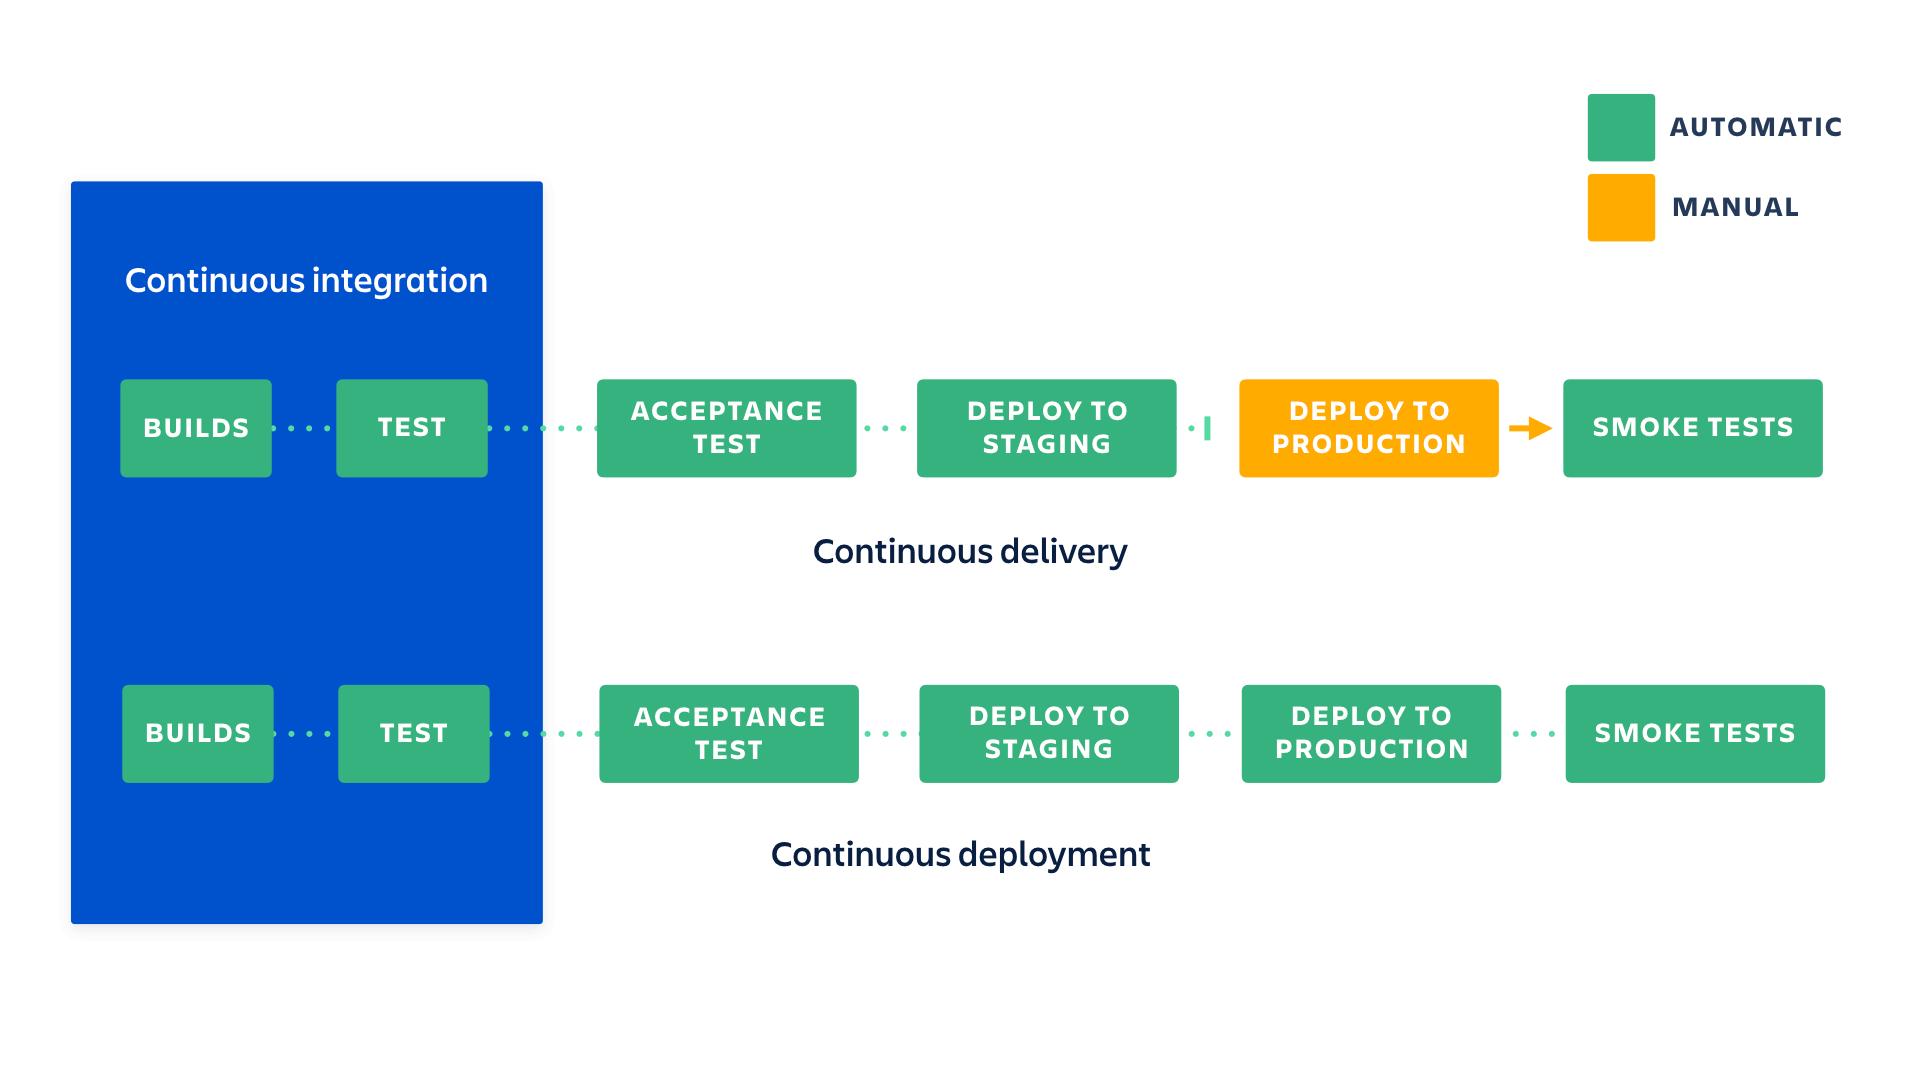
\includegraphics[width=0.51\textwidth]{./ci_cd_cd.png}
	\caption[CI \& CD]{CI \& CD\footnotemark}
	\label{fig_ci_cd}
\end{figure}
\footnotetext{\url{https://wac-cdn.atlassian.com/dam/jcr:b2a6d1a7-1a60-4c77-aa30-f3eb675d6ad6/ci\%20cd\%20asset\%20updates\%20.007.png?cdnVersion=508}}

In order to look into mobile approaches to CI/CD, it is first necessary to have a quick look into the "classical" theory. The original concept was heavily shaped by Kent Beck and Ron Jeffries in the context of their concept of Extreme Programming~\cite{beck1998extreme, beck2000extreme}

\subsection{Continuous Integration}
In his text about Continuous Integration Martin Fowler defined it as follows:

\begin{quoting}
"A software development practice where members of a team integrate their work frequently, usually each person integrates at least daily - leading to multiple integration per day. Each integration is verified by an automated build (including test) to detect integration errors as quickly as possible."~\cite{fowler2006continuous}
\end{quoting}

According to this, the typical workflow in a CI setup looks like the following. During the whole process there is always a high emphasis on monitoring the code state, checking (and preventing) broken code as often as possible. This process replaced the formerly used first-implement-then-integrate approach by integrating the code on a regular (daily) base.

\begin{itemize}
	\item Checkout master branch of repository
	\item Create working copy
	\item Add changes
	\item Check local build
	\item Verify integrity with local tests
	\item Downmerge with master branch
	\item Upmerge with master branch
	\item Automated build at server
	\item Automated testing at server
\end{itemize} 

Additional to this, he gave in the same text 9 practices to use CI. This list will be used in the following as a tool to analyze existing practices and especially to apply it for mobile CI/CD. 

\begin{enumerate}
	\item Maintain a Single Source Repository
	\item Automate the Build
	\item Make Your Build Self-Testing\footnote{\url{https://martinfowler.com/bliki/SelfTestingCode.html}}
	\item Everyone Commits Every Day
	\item Every Commit Should Build the Mainline on an Integration Machine
	\item Keep the Build Fast
	\item Test in a Clone of the Production Environment
	\item Make it Easy for Anyone to Get the Latest Executable
	\item Everyone can see what's happening
\end{enumerate}

\subsection{Continuous Delivery}

Coming from CI, Continuous Delivery builds upon this and adds additionally a manual deployment step to the production environment. So after every test runs through positively, the setup is ready to deploy by a click on a button at any time. But it still has a final human instance in between the push to the repository and the release.

\subsection{Continuous Deployment}

Removing the last human component in this process then leads to Continuous Deployment, making the full process fully automated. Each push the the master branch then automatically leads to a release deployment if the whole pipeline does not detect any failed tests or broken builds.

Disregarding if the last step is now fully automated or only partially with a final human component, I extend the mentioned checklist with:

\begin{enumerate}
	\item[10)] Automate Deployment
\end{enumerate}
